%===============================================================================
% LaTeX sjabloon voor de bachelorproef toegepaste informatica aan HOGENT
% Meer info op https://github.com/HoGentTIN/bachproef-latex-sjabloon
%===============================================================================

\documentclass{bachproef-tin}

\usepackage{hogent-thesis-titlepage} % Titelpagina conform aan HOGENT huisstijl
\graphicspath{{./img/}}

%%---------- Documenteigenschappen ---------------------------------------------
% TODO: Vul dit aan met je eigen info:

% De titel van het rapport/bachelorproef
\title{Het nut van pre-trained machine learning API's voor het classificeren van foto-archieven \protect\\ Een vergelijkende studie tussen Google Vision, AWS Rekognition en imagga}

% Je eigen naam
\author{Frederik Van Ruyskensvelde}

% De naam van je promotor (lector van de opleiding)
\promotor{Guy Dekoning}

% De naam van je co-promotor. Als je promotor ook je opdrachtgever is en je
% dus ook inhoudelijk begeleidt (en enkel dan!), mag je dit leeg laten.
\copromotor{Timon Devos}

% Indien je bachelorproef in opdracht van/in samenwerking met een bedrijf of
% externe organisatie geschreven is, geef je hier de naam. Zoniet laat je dit
% zoals het is.
\instelling{---}

% Academiejaar
\academiejaar{2020-2021}

% Examenperiode
%  - 1e semester = 1e examenperiode => 1
%  - 2e semester = 2e examenperiode => 2
%  - tweede zit  = 3e examenperiode => 3
\examenperiode{3}

%===============================================================================
% Inhoud document
%===============================================================================

\begin{document}

%---------- Taalselectie -------------------------------------------------------
% Als je je bachelorproef in het Engels schrijft, haal dan onderstaande regel
% uit commentaar. Let op: de tekst op de voorkaft blijft in het Nederlands, en
% dat is ook de bedoeling!

%\selectlanguage{english}

%---------- Titelblad ----------------------------------------------------------
\inserttitlepage

%---------- Samenvatting, voorwoord --------------------------------------------
\usechapterimagefalse
%%=============================================================================
%% Voorwoord
%%=============================================================================

\chapter*{\IfLanguageName{dutch}{Woord vooraf}{Preface}}
\label{ch:voorwoord}

%% TODO:
%% Het voorwoord is het enige deel van de bachelorproef waar je vanuit je
%% eigen standpunt (``ik-vorm'') mag schrijven. Je kan hier bv. motiveren
%% waarom jij het onderwerp wil bespreken.
%% Vergeet ook niet te bedanken wie je geholpen/gesteund/... heeft

Deze bachelorproef kwam tot stand als laatste uitdaging bij het voltooien van de opleiding Toegepaste Informatica, afstudeerrichting Mobile Apps. Als werkstudent en developer kwam ik via mijn job bij Docbyte de laatste jaren uitvoerig in contact met cloud platformen. Bij Docbyte worden de cloud tools ingeschakeld om documenten te lezen en nuttige informatie te extracten via computer vision modellen. Het viel mij meteen op dat deze modellen goed werkten voor tekst-extractie; ik wilde graag weten of ze ook goed werkten voor afbeeldingen.

De paper had niet tot stand kunnen komen zonder de hulpen van verschillende mensen. In de eerste plaats wil ik mijn promotor Guy Dekoning bedanken voor de correcte opvolging en boeiende feedback. Meneer Dekoning heeft steeds zijn best gedaan om meetings in te passen in mijn druk schema als werkstudent. Verder bedank ik graag mijn teamlead en co-promotor Timon Devos, Timon heeft mij over de jaren veel bijgeleerd en is in het proces een vriend geworden. Ook bedank ik graag Docbyte waar ik 3 jaar gewerkt heb en mijn stage heb gedaan, ze boden mij de kans om door te groeien binnen het bedrijf en waren steeds ondersteunend tijdens examenperiodes. 

Tot slot bedank ik het Archief Gent en de medewerkers van de Beeldbank\footnote{https://beeldbank.stad.gent/index.php} voor de interessante feedback en het voorzien van de testdata. De Beeldbank is een fascinerende bron van oude en nieuwe foto's, ik raad de lezers van deze paper aan om zeker eens een kijkje te nemen.
%%=============================================================================
%% Samenvatting
%%=============================================================================

% TODO: De "abstract" of samenvatting is een kernachtige (~ 1 blz. voor een
% thesis) synthese van het document.
%
% Deze aspecten moeten zeker aan bod komen:
% - Context: waarom is dit werk belangrijk?
% - Nood: waarom moest dit onderzocht worden?
% - Taak: wat heb je precies gedaan?
% - Object: wat staat in dit document geschreven?
% - Resultaat: wat was het resultaat?
% - Conclusie: wat is/zijn de belangrijkste conclusie(s)?
% - Perspectief: blijven er nog vragen open die in de toekomst nog kunnen
%    onderzocht worden? Wat is een mogelijk vervolg voor jouw onderzoek?
%
% LET OP! Een samenvatting is GEEN voorwoord!

%%---------- Nederlandse samenvatting -----------------------------------------
%
% TODO: Als je je bachelorproef in het Engels schrijft, moet je eerst een
% Nederlandse samenvatting invoegen. Haal daarvoor onderstaande code uit
% commentaar.
% Wie zijn bachelorproef in het Nederlands schrijft, kan dit negeren, de inhoud
% wordt niet in het document ingevoegd.

\IfLanguageName{english}{%
\selectlanguage{dutch}
\chapter*{Samenvatting}

\selectlanguage{english}
}{}

%%---------- Samenvatting -----------------------------------------------------
% De samenvatting in de hoofdtaal van het document

\chapter*{\IfLanguageName{dutch}{Samenvatting}{Abstract}}




%---------- Inhoudstafel -------------------------------------------------------
\pagestyle{empty} % Geen hoofding
\tableofcontents  % Voeg de inhoudstafel toe
\cleardoublepage  % Zorg dat volgende hoofstuk op een oneven pagina begint
\pagestyle{fancy} % Zet hoofding opnieuw aan

%---------- Lijst figuren, afkortingen, ... ------------------------------------

% Indien gewenst kan je hier een lijst van figuren/tabellen opgeven. Geef in
% dat geval je figuren/tabellen altijd een korte beschrijving:
%
%  \caption[korte beschrijving]{uitgebreide beschrijving}
%
% De korte beschrijving wordt gebruikt voor deze lijst, de uitgebreide staat bij
% de figuur of tabel zelf.

\listoffigures

% Als je een lijst van afkortingen of termen wil toevoegen, dan hoort die
% hier thuis. Gebruik bijvoorbeeld de ``glossaries'' package.
% https://www.overleaf.com/learn/latex/Glossaries

%---------- Kern ---------------------------------------------------------------

% De eerste hoofdstukken van een bachelorproef zijn meestal een inleiding op
% het onderwerp, literatuurstudie en verantwoording methodologie.
% Aarzel niet om een meer beschrijvende titel aan deze hoofstukken te geven of
% om bijvoorbeeld de inleiding en/of stand van zaken over meerdere hoofdstukken
% te verspreiden!

%%=============================================================================
%% Inleiding
%%=============================================================================

\chapter{\IfLanguageName{dutch}{Inleiding}{Introduction}}
\label{ch:inleiding}

Machine learning en AI (Artificiële Intelligentie) heeft het laatste decennium een grote sprong voorwaarts gemaakt. Er wordt al sinds de jaren 50 onderzoek gedaan naar een vorm van artificiële intelligentie maar door de noodzaak van complexe setups en benodigde compute power bleef AI eerder binnen de academische wereld en niet de bedrijfswereld. Sinds de opkomst van cloud computing wordt er echter een verandering waargenomen, steeds meer bedrijven kiezen ieder jaar voor de implementatie van een vorm van AI. Volgens een onderzoek gebaseerd op data van de US Census Bureau zou in 2018 3,5 procent van alle bedrijven in de Verenigde Staten AI reeds gebruiken of in testing hebben \autocite{Zolas2020}. Volgens de auteurs van dezelfde paper wordt er voorspeld dat AI een steeds grotere penetratie zal hebben in diverse bedrijfstakken.

\section{\IfLanguageName{dutch}{Probleemstelling}{Problem Statement}}
\label{sec:probleemstelling}
Op basis van deze evolutie lijkt het interessant om te onderzoeken of AI en machine learning kan toegepast worden op een concrete business case. Volgens \textcite{Zolas2020} gebruiken vooral grote bedrijven AI, het lijkt daarom interessant om te onderzoeken of ook een gemiddeld bedrijf gebruik kan maken van AI voor het oplossen van een concrete business case. Essentieel bij deze vraag is ease of use (of gemak van gebruik), een gemiddeld bedrijf moet de middelen en technische kennis in huis hebben vooropgesteld aan het gebruik van de AI. 

Bij het verfijnen van de onderzoeksvraag werd er gekozen om te focussen op het archiveren van foto's. Er zijn veel organisaties die grote foto-archieven hebben, zowel fysiek als digitaal, waarop niet gezocht kan worden. Met 'niet-zoekbare' foto-archieven wordt er begrepen dat er geen manier is om via een 'zoek'-functie de foto's te filteren op basis van inhoud. Het manueel zoekbaar maken van de foto-archieven is typisch een tijdrovend en vervelend werk, het automatiseren van dit proces zou voor grote tijdswinsten kunnen zorgen.

Het is belangrijk om op te merken dat foto-archieven een brede noemer is en dat het veel verschillende soorten foto's kan omvatten. Bijvoorbeeld foto's van gebouwen; landschappen; wildcamera's; kunstwerken; gezichten; wetenschapsonderwerpen; ...

Tot slot is het belangrijk dat accuraatheid van de AI voldoende hoog is,  in een productie-omgeving is het niet alleen belangrijk dat de foto's automatisch zoekbaar worden maar ook dat ze correct ingedeeld worden. Na besprekingen met archivarissen van Archief Gent en computer vision developers wordt er besloten om een foutmarge van 15\% toe te staan.

Uit de probleemstelling volgen 4 afgelijnde doelen:
\begin{itemize}
    \item Foto's zoekbaar maken door middel van AI
    \item De oplossing moet gemakkelijk te gebruiken zijn
    \item De oplossing moet breed bruikbaar zijn; voor veel verschillende soorten foto-archieven
    \item Foutmarge van maximaal 15\%
\end{itemize}

\section{\IfLanguageName{dutch}{Onderzoeksvraag}{Research question}}
\label{sec:onderzoeksvraag}
De onderzoeksvraag wordt opgebouwd op basis van de doelstellingen die uit de probleemstelling volgen.

Een specifieke tak binnen AI genaamd computer vision kan gebruikt worden om een computer te laten ''zien'' en bepaalde objecten op de foto te herkennen. De gevonden objecten kunnen dan gebruikt worden om de foto's zoekbaar te maken, dit proces heet classificatie. Er wordt dieper op deze onderwerpen ingegaan in Hoofdstuk \ref{ch:stand-van-zaken}.

Om de oplossing gemakkelijk bruikbaar te maken moet er een minimum aan configuratie en opzet nodig zijn bij het gebruik van de AI. Daarom werd er in dit onderzoek gekozen om enkel pre-trained API's te gebruiken. Pre-trained betekent dat het model reeds getraind werd en dat er geen configuratie door de consument moet gebeuren. Het gebruik van API's, in tegenstelling tot het gebruiken van lokale setup, zorgt opnieuwe voor een gemakkelijkere opzet - men kan stellen dat de meeste bedrijven de middelen ter beschikking hebben om te integreren met een API.

Om aan deze 3 doelen te voldoen werd er na inleidend onderzoek gekozen om de API's te gebruiken van de twee grootste spelers in het veld: Google Vision en Amazon AWS Rekognition en een kleinere speler genaamd imagga. Er wordt dieper op bovenstaande keuzes ingegaan in Hoofdstuk~\ref{ch:methodologie}.

Samengevat komen we tot de onderzoeksvraag: Het nut van pre-trained machine learning API's voor het classificeren van foto-archieven: Een vergelijkende studie tussen Google Vision, AWS Rekognition en imagga.

\section{\IfLanguageName{dutch}{Onderzoeksdoelstelling}{Research objective}}
\label{sec:onderzoeksdoelstelling}

Via een proof-of-concept wordt er al dan niet bewezen dat Google Vision en AWS Rekognition nuttig kunnen zijn bij het classificeren van foto-archieven. Uit dit resultaat wordt er een algemene conclusie getrokken rond het gebruik van pre-trained machine learning API's.

\section{\IfLanguageName{dutch}{Opzet van deze bachelorproef}{Structure of this bachelor thesis}}
\label{sec:opzet-bachelorproef}

% Het is gebruikelijk aan het einde van de inleiding een overzicht te
% geven van de opbouw van de rest van de tekst. Deze sectie bevat al een aanzet
% die je kan aanvullen/aanpassen in functie van je eigen tekst.

De rest van deze bachelorproef is als volgt opgebouwd:

In Hoofdstuk~\ref{ch:stand-van-zaken} wordt een overzicht gegeven van de stand van zaken binnen het onderzoeksdomein, op basis van een literatuurstudie.

In Hoofdstuk~\ref{ch:methodologie} wordt de methodologie toegelicht en worden de gebruikte onderzoekstechnieken besproken om een antwoord te kunnen formuleren op de onderzoeksvragen.

In Hoofdstuk~\ref{ch:resultaten} worden de resultaten van het onderzoek vergeleken.

% TODO: Vul hier aan voor je eigen hoofstukken, één of twee zinnen per hoofdstuk

In Hoofdstuk~\ref{ch:conclusie}, tenslotte, wordt de conclusie gegeven en een antwoord geformuleerd op de onderzoeksvragen. Daarbij wordt ook een aanzet gegeven voor toekomstig onderzoek binnen dit domein.
\chapter{\IfLanguageName{dutch}{Stand van zaken}{State of the art}}
\label{ch:stand-van-zaken}

% Tip: Begin elk hoofdstuk met een paragraaf inleiding die beschrijft hoe
% dit hoofdstuk past binnen het geheel van de bachelorproef. Geef in het
% bijzonder aan wat de link is met het vorige en volgende hoofdstuk.

% Pas na deze inleidende paragraaf komt de eerste sectiehoofding.
Deze bachelorproef onderzoekt of machine learning engines gebruikt kunnen worden voor het automatisch classificeren van afbeeldingen. In deze stand van zaken komen volgende onderwerpen aan bod:
\begin{enumerate}
    \item Classificeren van afbeeldingen: terminologie en technieken
    \item Bespreking belangrijkste stromingen binnen machine learning
    \item Computer vision: hoe wordt classificatie en machine learning gecombineerd
\end{enumerate}

\section{\IfLanguageName{dutch}{Classificeren van afbeeldingen}{Image classification}}
\label{sec:classificeren-van-afbeeldingen}
Voor er dieper in gegaan wordt op machine learning en hoe deze algoritme's kunnen toegepast worden om computers te laten 'zien' is het belangrijk om te bespreken hoe classificatie van afbeeldingen gebeurt.

Het classificeren van afbeeldingen kan gedefinieerd worden als het groeperen van afbeeldingen in semantisch betekenisvolle categorien op basis van onderdelen van de afbeeldingen \autocite{Vailaya1998}. Deze ''semantisch betekenisvolle categorieën'' worden ook labels genoemd, voorbeelden van labels zijn 'fiets', 'landschap', 'blijdschap'. Het is belangrijk om te vermelden dat labels zowel objecten kunnen zijn maar ook meer algemene of abstracte concepten. Verder kunnen labels meer of minder gedetailleerd zijn, denk bijvorbeeld aan 'mens'; 'gezicht'; 'oog'; 'pupil'; ... Het correct aanduiden van labels is een belangrijk probleem wanneer men grote datasets van afbeeldingen zoekbaar wilt maken, bijvoorbeeld foto-archieven of medisch beeldmateriaal. Deze labels worden typisch niet in de afbeelding zelf opgeslaan maar in een bijhorend metadata bestand; wanneer er metadata voor een afbeelding beschikbaar is spreekt men van een verrijkte afbeelding.

Naast het zoeken van labels voor een afbeelding kan men ook eventuele tekst op de afbeelding lezen en deze toevoegen aan de metadata, opnieuw wordt op deze manier de afbeelding verrijkt. Bijvoorbeeld het woord 'Politie' bij een foto van een politie-kantoor.

In de volgende secties wordt manuele (of mens-gestuurde) en automatische (of computer-gestuurde) classificatie meer in detail besproken.

\subsection{\IfLanguageName{dutch}{Manuele classificatie}{Manual classification}}
\label{sec:manuele-classificatie}
Manuele classificatie wordt gedefinieerd als het toewijzen van labels aan een afbeelding, uitgevoerd door een mens. Het manueel classificeren van afbeeldingen is een tijdrovend proces. Iedere afbeelding moet door een persoon geopend worden, deze persoon bekijkt de afbeelding en verrijkt de afbeelding aan de hand van labels. Voor het classificeren van miljoenen of miljarden afbeeldingen is manuele classificatie zeer tijdsintensief en wordt er vaak naar automatische opties gezocht. Automatische of computergestuurde modellen hebben echter steeds manueel gelabelde datasets als trainingsmateriaal dus is het cruciaal dat de kwaliteit van deze manueel geclassificeerde datasets hoog is \autocite{JuliaMoehrmann2012}.

Er werd reeds veel onderzoek en ontwikkeling verricht naar hoe men mensen kan helpen afbeeldingen op een snelle en correcte manier te labelen. Bijvoorbeeld via geavanceerde interfaces \autocite{JuliaMoehrmann2012} of gamification \autocite{LuisvonAhn2004}. Een voorbeeld van manuele classificatie is het invullen van een CAPTCHA, de manuele input van deze beveiligingstechnologie wordt door Google gebruikt om machine learning modellen te trainen \autocite{Google2021}, zie Figuur~\ref{fig:captcha}.

\begin{figure}
    \centering    
    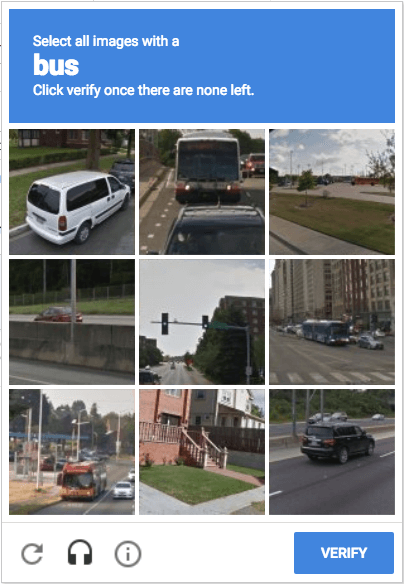
\includegraphics[scale=0.5]{recaptcha}
    \caption{CAPTCHA's worden als input gebruikt voor machine learning modellen. Bron: \url{https://auth0.com/blog/captcha-can-ruin-your-ux-here-s-how-to-use-it-right}}
    \label{fig:captcha}
\end{figure}

\subsection{\IfLanguageName{dutch}{Automatiche classificatie}{Automatic classification}}
\label{sec:automatic-classification}
Onder automatische classificatie begrijpen we het toewijzen van labels aan een afbeelding zonder menselijke input. Een computermodel krijgt een afbeelding aangeboden en wijst aan deze afbeelding verschillende labels toe. Aan iedere label zal een zekerheidsgraad meegegeven worden, uitgedrukt in procent. De computermodellen worden steeds getraind op basis van manueel geclassificeerde afbeeldingen, ook controle van de resultaten gebeurt door menselijke supervisie. Er is dus steeds een samenwerking tussen mens en machine. Typisch worden er machine learning modellen gebruikt om automatische classifictie zo correct mogelijk toe te passen.

Bij het automatisch classificeren van afbeeldingen kan men ook Optical Character Recognition (OCR) uitvoeren. OCR engines zullen proberen tekst te herkennen op een afbeelding en deze toevoegen aan de metadata. Het uitvoeren van kwalitatieve OCR is een apart vakgebied binnen machine learning waar er de laatste jaren veel vooruitgang werd geboekt, een belangrijk probleem in dit veld is het herkennen van handgeschreven tekst \autocite{Breuel2013}.

\section{\IfLanguageName{dutch}{Machine learning}{machine learning}}
\label{sec:machine-learning}
Machine learning is een bepaalde soort computer algoritme dat ontworpen werd om menselijke intelligentie te emuleren door bij te leren uit de directe omgeving \autocite{ElNaqa2015}. Op basis van vroegere ervaringen zal het algoritme trachten om efficientie te verhogen of correcte voorspellingen te maken. In deze context wordt ervaring gedefinieerd als informatie die voor het systeem beschikbaar is, typisch in de vorm van elektronische data. Deze elektronische data kan verschillende vormen aannemen, bijvoorbeed datasets gelabeld door mensen of data gegeneerd door andere machines op basis van hun contact met de buitenwereld. De hoeveelheid en kwaliteit van de data zal steeds cruciaal zijn voor de performantie van het machine learning algoritme \autocite{Mohri2018}.

Machine learning algoritmes bieden computer de mogelijkheid om te leren zonder expliciet geprogrammeerd te zijn \autocite{DeVreese2017}. De problemen waarvoor machine learning meestal gebruikt wordt zijn te complex om via klassieke programmeertechnieken aan te pakken. Aangezien machine learning slechts een techniek is waarmee men tracht complexe problemen op te lossen werd het succesvol gebruikt in uiteenlopende onderzoeksvelden zoals ruimtevaart, statistiek, biomedica en computer vision.

Machine learning algoritmes kunnen in het algmeen opgedeeld worden in 3 type's:
\begin{itemize}
    \item Supervised learning
    \item Unsupervised learning
    \item Reinforcement learning
\end{itemize}

\subsection{\IfLanguageName{dutch}{Supervised learning}{Supervised learning}}
\label{sec:supervised-learning}
De belangrijskte karakteristiek van supervised learning is dat het machine learning algoritme een vooraf gelabelde trainingsdataset ter beschikking heeft. Supervised learning zal op basis van deze trainingsdataset trachten, door middel van inductie, modellen op te bouwen die gebruikt kunnen worden om andere ongelabelde datasets te classificeren. Achteraf kan dan gecontroleerd worden hoeveel percent van de nieuwe labels correct werd gevonden en hoe zeker het model was van deze voorspellingen. Zoals de naam van het model aangeeft is er een vorm van een 'supervisor' nodig die het model toont welke labels met welke ervaringen uit de trainingsdata moeten geassocieerd worden \autocite{Cunningham2008}. 

Een voorbeeld van supervised learning is hoe Netflix nieuwe content aan de users voorstelt. Het algoritme start van een gelabelde dataset met daarin de ervaringen van de gebruiker, op basis van deze ervaringen zal het model voorspellingen over nieuwe content maken.

\subsection{\IfLanguageName{dutch}{Unsupervised learning}{Unsupervised learning}}
\label{sec:unsupervised-learning}
In tegenstelling tot supervised learning wordt er bij unsupervised learning vertrokken van een ongelabelde dataset. Het doel is dat het algoritme deze ongelabelde dataset zal intepreteren en een interne representatie van de 'wereld' - de 'wereld' is alle informatie binnen de dataset - zal opbouwen. Een unsupervised learning model zal proberen een diepe kennis van de wereld op te bouwen aan de hand van complexe patroonherkenning \autocite{Hinton1999}. Op basis van deze diepere kennis zal het algoritme de data in verschillende clusters onderverdelen. Analyse van deze clusters kan dan leiden tot het labellen of classificeren van de ongelabelde dataset.

Unsupervised learning wordt in verschillende bedrijfstakken actief toegepast, Google News gebruikt bijvoorbeeld unsupervised learning om nieuwsartikelen rond hetzelfde nieuwsfeit automatisch te clusteren en op een georganiseerde manier aan de gebruiker aan te bieden.

\subsection{\IfLanguageName{dutch}{Reinforcement learning}{Reinforcement learning}}
\label{sec:reinforcement-learning}
Reinforcement learning is een machine learning algoritme dat steeds zal zoeken naar een zo hoog mogelijke beloning, uitgedrukt in een numerieke waarde. Het algoritme krijgt op voorhand geen uitleg wat goed of fout is maar moet zelf ontdekken welke acties leiden tot de grootst mogelijke beloning \autocite{Sutton2018}. Uit het iteratief uitvoeren van dezelfde opdracht en ontvangen van een beloning zal het algoritme een duidelijk beeld krijgen welke acties de grootste beloning opleveren. Het zal steeds een balans moeten houden tussen exploratief onderzoeken en in de diepte onderzoeken van reeds gevonden oplossingen. 

Reinforcement learning vindt toepassingen in verschillende sectoren zoals autonoom auto-rijden, handelen op de aandelenmarkt en gaming. Reinforcement learning sluit inherent dicht aan bij gaming dat met dezelfde soort trial-and-error beloningssystemen werkt, bijgevolg werd er reeds veel onderzoek verricht naar het gebruik van reinforcement learning om spelletjes te spelen. Een voorbeeld uit 2015 is een wedstrijd van het complexe bordspel Go tussen wereldkampioen Fan Hui en AlphaGo. AlphaGo is een algoritme ontwikkeld door Google, gebaseerd op het reinforcement learning principe. Fan Hui verloor de match met 1-4, het was de eerste keer dat een computer-gestuurd programma een Go wereldkampioen versloeg.

\begin{figure}
    \centering
    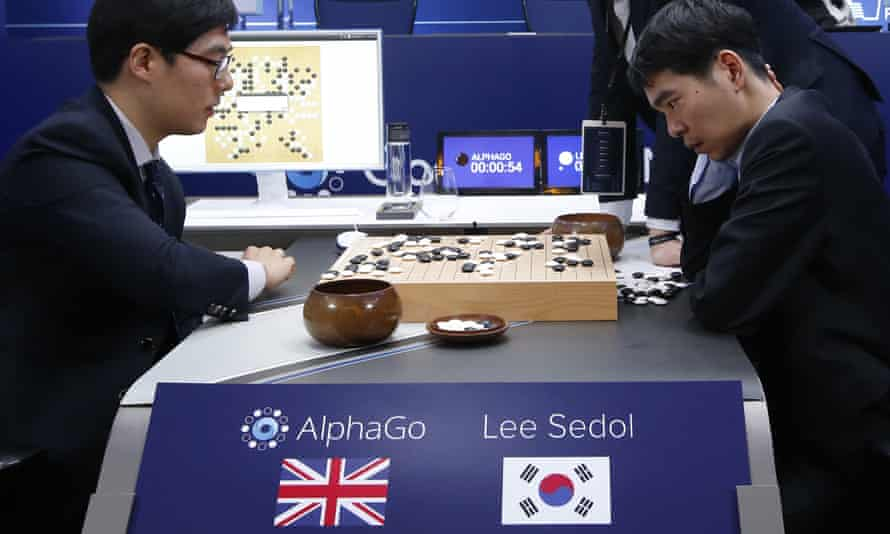
\includegraphics[width=\textwidth]{alphago}
    \caption{Wereldkampioen Fan Hui speelt tegen AlphaGo. Bron: \url{https://www.theguardian.com/technology/2016/mar/15/alphago-what-does-google-advanced-software-go-next}}
    \label{fig:alphago}
\end{figure}

\section{\IfLanguageName{dutch}{Computer vision}{Computer vision}}
\label{sec:computer-vision}
Computer vision wordt begrepen als de combinatie van technieken die gebruikt wordt om complexe hoger-dimensionale data (afbeeldingen) te analyseren en verwerken \autocite{Jaehne2000}. De meest gebruikte machine learning strategieën bij computer vision zijn supervised, unsupervised en semi-supervised \autocite{Khan2020}. Binnen de supervised learning subset wordt computer vision gedefinieerd als een deep learning model. Deep learning betekent dat er gebruikt wordt gemaakt van een neuraal netwerk met ten minste 3 of meer lagen. Een neuraal netwerk is een serie algoritme's die probeert om onderlinge relaties in een dataset te herkennen, het menselijk brein kan ook als een neuraal netwerk gedefinieerd worden.

\subsection{\IfLanguageName{dutch}{Hoe kan een computer 'zien'}{How does a computer 'see'}}
\label{sec:how-do-computer-see}

Voor mensen is zicht en herkenning van de wereld rond ons een normaal en natuurlijk proces. Licht wordt weerkaatst door een object en opgevangen door de ogen, de ogen geven deze data door naar de visuele cortex die het beeld interpreteert. Door middel van miljoenen jaren evolutie werd ons brein getrained in het zien en interpreteren van de wereld. Essentieel is dat iedere mens een bepaald idee heeft van de wereld die de beelden die van de ogen komen betekenis geeft. Dit 'idee van de wereld' wordt ook als context gedefinieerd, zonder context kan een afbeelding geen betekenis hebben.
Bijvoorbeeld als een alien een foto te zien zou krijgen die gemaakt werd op de aarde, zal het voor hem moeilijk zijn om de foto te 'begrijpen' omdat de context ontbreekt.

Het ontbreken van context is wat het voor computers ook heel moeilijk maakt om te herkennen wat er op een afbeelding staat. Voor een computer ziet een afbeelding er typisch uit als Figuur~\ref{fig:pixelarray}, een lijst van integers. De computer weet hoe het deze integers moet omvormen tot een afbeelding, maar heeft geen informatie over de inhoud van de afbeelding.

\begin{figure}
    \centering
    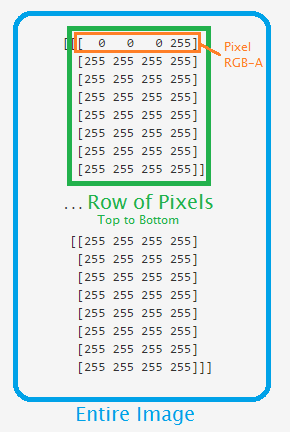
\includegraphics[scale=1]{pixelarray}
    \caption{Voorbeeld van hoe een afbeelding er voor een computer uit ziet. Bron: \url{https://pythonprogramming.net/python-pixel-arrays/}}
    \label{fig:pixelarray}
\end{figure}

Computer vision gebruikt verschillende strategien om context rond een afbeelding op te bouwen, eerst zullen de algoritme's proberen om vormen en figuren te herkennen op de afbeelding. Wanneer deze vormen en figuren gedefinieerd zijn zal men op basis van pre-gelabelde datasets de betekenis van deze figuren afleiden. Op de meeste vlakken heeft computer vision het nadeel van het ontbreken van context, maar in sommige gevallen kan dit net in het voordeel van herkenning spelen. Als men een ingezoomde foto met erop de vacht van een bepaald dier aan een mens toont, zal het vaak moeilijk zijn om het dier te herkennen. Een computer vision algoritme zou kunnen het patroon van de vacht berekenen en op basis hiervan in de pre-geclassificeerde dataset de diersoort opzoeken. Het ontbreken van context speelt hier niet in het nadeel van computer vision.

Na miljoenen jaren natuurlijke evolutie van het zicht zijn we nu op een interessant punt waarbij computer vision steeds dichter bij de menselijke herkenningsskills komt \autocite{Scheirer2014}. In de toekomst zal computer vision waarschijnlijk accurater worden dan het menselijk zicht.

\subsection{\IfLanguageName{dutch}{Convolutional neural network}{Convolutional neural network}}
\label{sec:convolutional-neural-network}
Achterliggend zal men bij computer vision meestal een Convolutional Neural Network (CNN) gebruiken, dit is een bepaald subtype van supervised deep learning. CNN werkt door afbeeldingen op te delen in kleinere groepjes pixels die men filters of feature maps noemt. Deze filters worden door de lagen van het neuraal netwerk doorgegeven, in de eerste lagen zal men proberen om algemene informatie te herkennen zoals randen of vormen. De output van iedere laag wordt aan de volgende doorgegeven, tijdens het doorgeven van het resultaat wordt iedere filter afgecheckt tegen tegen een pre-geclassificeerde trainingsdataset. Het afchecken geeft aan het CNN een bepaalde error-waarde (ofwel loss function) terug, deze error-waarde geeft aan hoe groot de kans is dat er iets herkend wordt. Op basis van deze error-waarde zal het algoritme bij iedere iteratie de filtervalues updaten. Idealiter zal iedere iteratie een betere error-waarde opleveren. Op het einde van het proces wordt alle opgebouwde kennis gepooled tot het herkennen van complexe en abstracte begrippen, zie Figuur~\ref{fig:cnn} voor een overzicht.

\begin{figure}
    \centering
    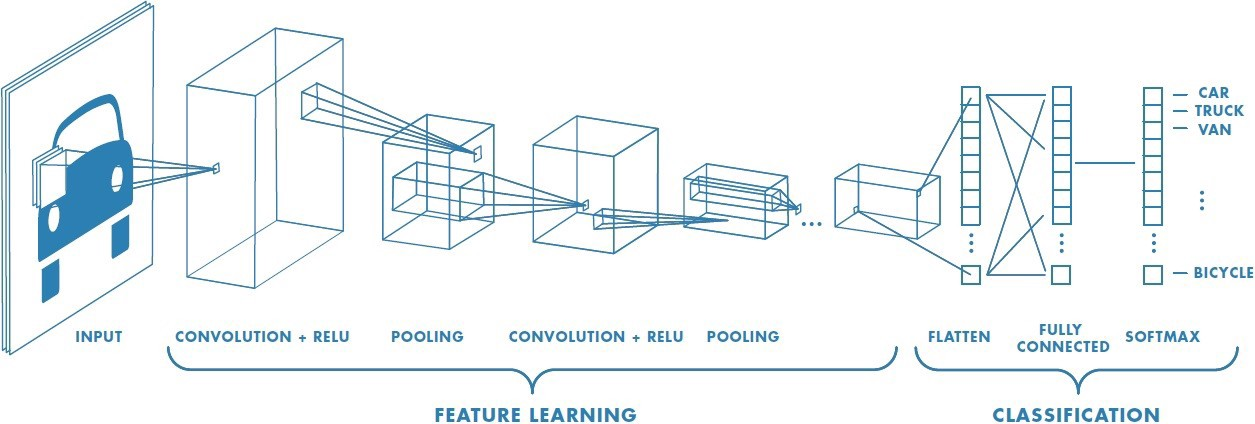
\includegraphics[width=\textwidth]{cnn}
    \caption{Een Convolutional Neural Network (CNN). Bron: \url{https://towardsdatascience.com/a-comprehensive-guide-to-convolutional-neural-networks-the-eli5-way-3bd2b1164a53}}
    \label{fig:cnn}
\end{figure}

Een uitdaging bij dit soort modellen is dat men zeer grote hoeveelheden data nodig heeft (miljoenen afbeeldingen) voor men accuraat labels kan voorspellen \autocite{Chen2014}. Het is belangrijk dat het model van iedere label meerdere voorbeelden heeft, bijvoorbeeld als een model getrained wordt met een afbeelding van een eend en het krijgt slechts 1 afbeelding van een eend; dan zal het model ook de achtergrondkleur en belichting als essentiele informatie van de foto beschouwen. Wanneer men een afbeelding van een andere eend met andere belichting aanbiedt, zal het model dit niet als eend herkennen. Aansluitend is het belangrijk dat de trainingsdataset correct gelabeld is.

\subsection{\IfLanguageName{dutch}{Recurrent neural network}{Recurrent neural network}}
\label{sec:recurrent-neural-network}
Wanneer men videobeelden wilt analyseren kan men in essentie iedere frame nemen en analyseren met CNN zoals bij een gewone afbeelding. Het probleem is echter dat iedere afbeelding op zich wordt geanalyseerd en dat het CNN geen weet heeft van de relatie tussen de vorige en de volgende frames. Hierdoor geraakt belangrijke context-informatie verloren die gebruikt moet worden om correcte voorspellingen te maken.
Dit probleem kan men oplossen door de output van het CNN in een 'temporally sensitive model' ofwel een Recurrent Neural Network (RNN) te feeden.

In tegenstelling tot CNN kan RNN informatie onthouden over de vorige reeds geidentificeerde afbeeldingen en dit gebruiken bij het maken van toekomstige beslissingen, zie Figuur~\ref{fig:rnn}.

\begin{figure}
    \centering
    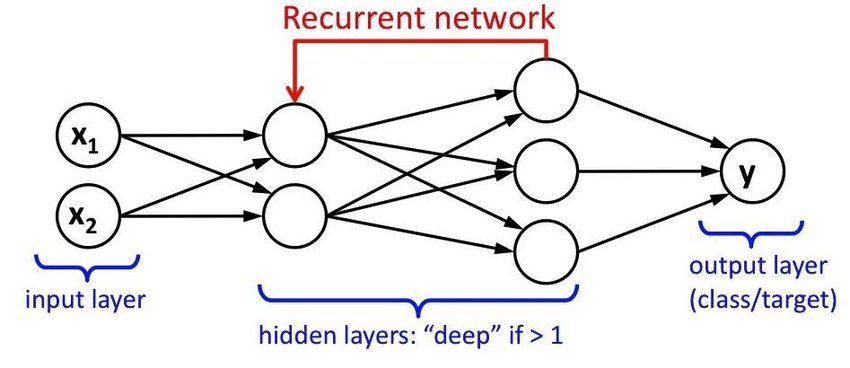
\includegraphics[width=\textwidth]{rnn}
    \caption{Een Recurrent Neural Network (RNN). Bron: \url{https://www.researchgate.net/figure/Recurrent-neural-networkRNN-or-Long-Short-Term-MemoryLSTM-5616_fig2_324883736}}
    \label{fig:rnn}
\end{figure}
%%=============================================================================
%% Methodologie
%%=============================================================================

\chapter{\IfLanguageName{dutch}{Methodologie}{Methodology}}
\label{ch:methodologie}

%% TODO: Hoe ben je te werk gegaan? Verdeel je onderzoek in grote fasen, en
%% licht in elke fase toe welke stappen je gevolgd hebt. Verantwoord waarom je
%% op deze manier te werk gegaan bent. Je moet kunnen aantonen dat je de best
%% mogelijke manier toegepast hebt om een antwoord te vinden op de
%% onderzoeksvraag.

\lipsum[21-25]


%%=============================================================================
%% Resultaten
%%=============================================================================

\chapter{\IfLanguageName{dutch}{Resultaten}{Results}}
\label{ch:resultaten}

\section{\IfLanguageName{dutch}{Inleiding}{Preface}}
\label{sec:resultaten-inleiding}
Na het uitvoeren van de code zoals besproken in Hoofdstuk\ref{ch:methodologie} werd er een csv\footnote{https://docs.google.com/spreadsheets/d/1vGC7rQ9PlnfjhAAsU6fJdlmlrZMXW1S3uCMdqmFghqI} gegenereerd waarbij voor iedere afbeelding in de dataset 3 labels werden opgehaald bij de respectievelijke API's.

Op basis van deze csv werd voor iedere label een score vastgelegd zoals besproken in Sectie~\ref{sec:scoren-van-labels}. Daarnaast werd voor ieder gevonden label aangeduid of de threshold van 75\% zekerheidsgraad gehaald werd, de volledige resultaten van de scoring kunnen teruggevonden worden in deze\footnote{https://docs.google.com/spreadsheets/d/1oCs-aDkhPV2lCayjLyzUPF0SlAUZ7vMjzD4DYuIluyE} Google Sheet. In de sheet kan men ook de aggregatie van de resultaten en grafieken terugvinden.

In de eerste sectie van dit hoofdstuk worden de resultaten besproken waarbij labels met een zekerheidsgraad onder de threshold genegeerd werden. In de volgende sectie worden de volledige resultaten van het onderzoek besproken en wordt de impact van de threshold per computer vision API verder toegelicht. Ten slotte wordt de peformantie van iedere API besproken en wordt er een besluit getrokken in functie van de onderzoeksvraag.

\section{\IfLanguageName{dutch}{Resultaten met thresholding}{Results with thresholding on confidence}}
\label{sec:resultaten-met-thresholding}
In de genormaliseerde staafdiagram op Figuur~\ref{fig:resultswiththresholding} worden het aantal resultaten per score van iedere computer vision API afgebeeld, waarbij de labels met een zekerheidsgraad onder 75\% werden genegeerd. Figuur~\ref{fig:resultswiththresholdingnotstacked} beeldt dezelfde data af maar in absolute waardes.

\begin{figure}
    \centering    
    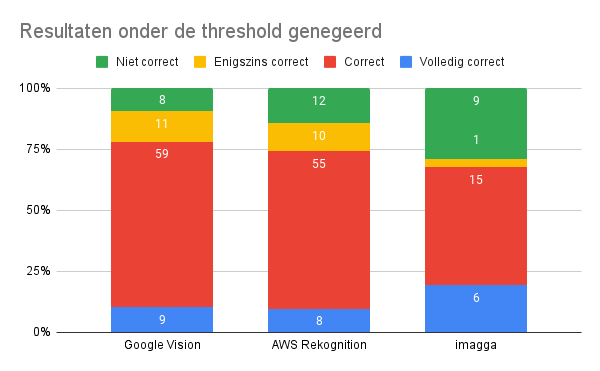
\includegraphics[width=\textwidth]{resultswiththresholding}
    \caption{Resultaten label-herkenning per API, met thresholding}
    \label{fig:resultswiththresholding}
\end{figure}

\begin{figure}
    \centering    
    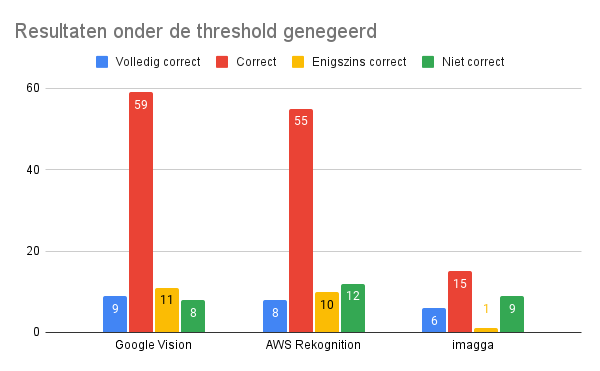
\includegraphics[width=\textwidth]{resultswiththresholdingnotstacked}
    \caption{Resultaten label-herkenning per API, met thresholding niet genormaliseerd}
    \label{fig:resultswiththresholdingnotstacked}
\end{figure}

Bij zowel Google Vision als AWS Rekognition zijn de resultaten gelijkaardig, imagga scoort significant verschillend. Aangezien de resultaten van Google Vision en AWS Rekognition dicht bij elkaar liggen worden deze naast elkaar besproken. Bij beide API's is het grootste deel van de gevonden labels 'correct'. Dit betekent dat de label correct was voor de afbeelding maar niet in de originele dataset vervat zat. Verder wijken ook de scores van van 'volledig correct' en 'engiszins correct' niet van elkaar significant af. Bij Google Vision werden er 8 labels - of 9,2\% van het totaal- als 'niet correct' gepunt, AWS Rekognition scoort hier 12 verkeerde labels of 14,12\% van het totaal. Een verschil minder dan 5\% is niet significant maar kan een trend voorspellen.

In Figuur~\ref{fig:resultsthresholding} wordt het aantal labels afgebeeld dat de threshold-zekerheidsgraad niet haalde, opnieuw zien we een niet significant verschil tussen Google Vision en AWS Rekognition. Bij Google Vision vielen 3 labels of 3,3\% van het totaal onder de threshold, bij AWS Rekognition is dat 5 labels of 5,6\% van het totaal. Men kan stellen dat de resultaten over de hele lijn sterk gelijkaardig zijn tussen Google Vision en AWS Rekognition, met de mogelijkheid dat Google Vision iets beter scoort.

\begin{figure}
    \centering    
    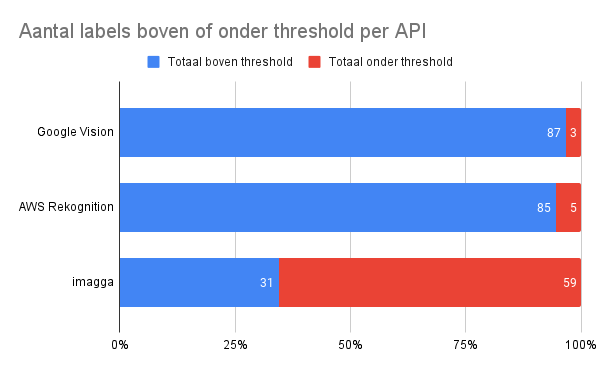
\includegraphics[width=\textwidth]{resultsthresholding}
    \caption{Aantal labels boven of onder de threshold per API}
    \label{fig:resultsthresholding}
\end{figure}

De resultaten van imagga geven een ander beeld, bij Figuur~\ref{fig:resultswiththresholdingnotstacked} is op het eerste zich duidelijk dat er minder resultaten beschikbaar zijn als bij Google Vision of AWS Rekognition. Dit komt omdat 59 van de 90 labels (of 65,6\%) onder de threshold vallen, dit zorgt voor slechts 31 resultaten die geanalyseerd kunnen worden.

Opvallend is dat voor imagga het aantal labels met 'volledig correct' een significant hoger percentage (19,35\%) van het totaal omvat als voor Google Vision (10,34\%) of AWS Rekognition (9,41\%). Verder heeft imagga slechts 1 'engiszins correct' label. 9 labels of 29,03\% van het totaal werden gescoord als 'niet correct', dit is een significant verschil met de 'niet correct' scores van Google Vision en AWS Rekognition. Aangezien er voor imagga procentueel gezien veel labels als 'volledig correct' en 'niet correct' werden aangeduid maar weinig labels als 'enigszins correct' kan men stellen dat het model ofwel zeer correct is, ofwel volledig verkeerd is. 15 labels of 48,39\% van het totaal werden voor imagga als 'correct' aangeduid, opnieuw is dat een significant lager percentage vergeleken met Google Vision (67,8\%) en AWS Rekognition (64,7\%).

Verder viel bij het analyseren van de resultaten op dat imagga de enige API is die zekerheidsgraden van 100\% terug geeft, opnieuw kan men stellen dat imagga ofwel heel zeker is of helemaal niet zeker. De zekerheidsgraden van Google Vision en AWS Rekognition bevinden zich meestal tussen 85\% en 99.9\%.

\section{\IfLanguageName{dutch}{Resultaten zonder thresholding}{Results without thresholding}}
\label{sec:resultaten-zonder-thresholding}
In Figuur~\ref{fig:resultswithoutthresholding} worden de opgetelde scores per API genormaliseerd afgebeeld, zonder dat de scores onder de threshold werden genegeerd.

Het verschil in scores tussen Google Vision en AWS Rekognition is opnieuw niet significant, dit is logisch te verklaren omdat bij beide API's slechts enkele labels onder de threshold vielen. Bij imagga wordt er echter belangrijke significante verschillen opgemerkt, er zijn 27 meer 'correct' labels en 26 meer 'niet correct' labels. Procentueel gezien stijgt 'niet correct' met 9,1\% en daalt 'volledig correct' met 11,6\% de andere scores zijn niet significant verschillend.

Er kan gesteld worden dat imagga veruit het meest terughoudend is met de zekerheidgraad, een correct manier van labelen aangezien het accepteren van een lagere zekerheidsgraad procentueel gezien tot meer verkeerde resultaten leidt.

\begin{figure}
    \centering    
    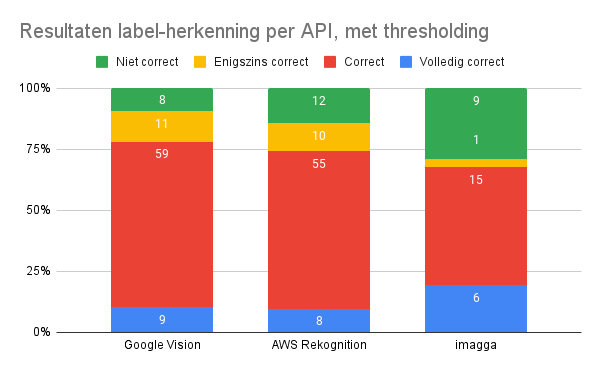
\includegraphics[width=\textwidth]{resultswithoutthresholding}
    \caption{Resultaten label-herkenning per API, zonder thresholding}
    \label{fig:resultswithoutthresholding}
\end{figure}

\section{\IfLanguageName{dutch}{Snelheid per API}{Speed per api}}
\label{sec:snelheid-per-api}
Alhoewel snelheid van verwerking geen belangrijk doel is in de use-case van deze Bachelorproef wordt ze toch kort geanalyseerd als bijkomstige informatie. 
Van iedere call werd bijgehouden hoe snel labels geretourneerd worden, deze data werd verwerkt tot gemiddeldes:

\begin{enumerate}
    \item Classificeren van afbeeldingen: terminologie en technieken
    \item Bespreking belangrijkste stromingen binnen machine learning
    \item Computer vision: hoe wordt classificatie en machine learning gecombineerd
\end{enumerate}

\section{\IfLanguageName{dutch}{Besluit}{Resolution}}
\label{sec:besluit}

% Voeg hier je eigen hoofdstukken toe die de ``corpus'' van je bachelorproef
% vormen. De structuur en titels hangen af van je eigen onderzoek. Je kan bv.
% elke fase in je onderzoek in een apart hoofdstuk bespreken.

%\input{...}
%\input{...}
%...

%%=============================================================================
%% Conclusie
%%=============================================================================

\chapter{Conclusie}
\label{ch:conclusie}

% TODO: Trek een duidelijke conclusie, in de vorm van een antwoord op de
% onderzoeksvra(a)g(en). Wat was jouw bijdrage aan het onderzoeksdomein en
% hoe biedt dit meerwaarde aan het vakgebied/doelgroep? 
% Reflecteer kritisch over het resultaat. In Engelse teksten wordt deze sectie
% ``Discussion'' genoemd. Had je deze uitkomst verwacht? Zijn er zaken die nog
% niet duidelijk zijn?
% Heeft het onderzoek geleid tot nieuwe vragen die uitnodigen tot verder 
%onderzoek?

Zoals besproken in het vorige hoofdstuk wordt het duidelijk dat zowel Google Vision als AWS Rekognition bruikbaar zijn om de probleemstelling aan te pakken. De API's kunnen op snel tempo, met een hoge mate van zekerheid, labels aan verschillende soorten afbeeldingen toewijzen. De setup en configuratie is minimaal en kan door een gemiddeld bedrijf opgezet worden. Idealiter wordt er een front-end rond een of meerdere van deze API's gebouwd en kan een gewone PC gebruiker automatische labeling laten uitvoeren. Deze Bachelorproef kan als leidraad dienen voor organisatie's die foto-archieven hebben en deze op een correcte en gemakkelijke manier willen labelen. 
De imagga API scoorde niet voldoende hoog genoeg gebruikt te worden voor deze doelstellingen.

De labeling door API's heeft een hoge mate van correctheid (\char`\~ 90\%), toch schieten de API's momenteel op 1 vlak duidelijk te kort: het ontbreken van context. Context zorgt er voor dat een persoon aan de hand van de volledige informatie vervat in de afbeelding correct kan inschatten welke labels er toepasbaar zijn. De computer vision API's ontbreken deze context volledig en geven bijgevolg regelmatig labels die te algemeen zijn en weinig waarde toevoegen. Het is dan ook belangrijk om te benadrukken dat de API's besproken in deze studie manuele classificatie niet kunnen vervangen, het is interessanter om ze als een hulpmiddel te zien die archivarissen kunnen helpen om foto's sneller te labelen. Aangezien de API's een foutmarge van \char`\~ 10\% hebben is het belangrijk dat een persoon de gevonden labels controleert.

Na eerdere ervaringen met computer vision modellen werd deze uitkomst verwacht, het is duidelijk dat AI momenteel veel kan maar nog niet op het niveau van de menselijke kennis staat. Het laatste decennium heeft computer vision grote sprongen voorwaarts gemaakt, het zou dan ook interessant om een soortegelijk onderzoek opnieuw uit te voeren binnen 5 à 10 jaar. Verder onderzoek kan zich ook focussen op het dieper onderzoeken van de zekerheidsgraad threshold; welke threshold zorgt er voor de hoogste scores per API.

%%=============================================================================
%% Bijlagen
%%=============================================================================
  
\appendix
\renewcommand{\chaptername}{Appendix}

%%---------- Onderzoeksvoorstel -----------------------------------------------

\chapter{Onderzoeksvoorstel}

Het onderwerp van deze bachelorproef is gebaseerd op een onderzoeksvoorstel dat vooraf werd beoordeeld door de promotor. Dat voorstel is opgenomen in deze bijlage.

% Verwijzing naar het bestand met de inhoud van het onderzoeksvoorstel
%---------- Inleiding ---------------------------------------------------------

\section{Introductie} % The \section*{} command stops section numbering
\label{sec:introductie}
In het laatste decenium is data-generatie en -verwerking steeds meer op de voorgrond getreden. Moderne ondernemingen proberen zo veel mogelijk data digitaal te genereren en op te slaan - zonder dat daar fysieke documenten aan te pas komen. Een groot deel van de ondernemingen heeft echter naast het digitaal archief nog steeds een papieren archief.
Digitalisatie van documenten is van cruciaal belang om gemakkelijker de huidige stand van zaken te analyseren en om toekomstige trends te voorspellen. In verschillende sectoren wordt er daarom steeds meer ingezet op digitalisatie van deze papieren archieven \autocite{PekkaLeviaekangas2020}. 

Binnen het vakgebied digitale archiveringen wordt er veelal gefocused op het archiveren van documenten met tekst op basis van OCR (Optical Character Recognition). Met OCR wordt geprobeerd om tekst op afbeeldingen om te zetten naar tekst in string vorm. Aangezien de meeste foto's geen tekst bevatten die nuttig zijn voor het categoriseren van de foto kunnen de OCR technieken niet op dit vakgebied toegepast worden.

Digitale foto's werden pas populairder dan fysieke foto's rond het jaar 2000 \autocite{HenryC.LucasJr.2009} - er zijn dus ongewtijfeld ondernemingen die met niet-gedigitaliseerde foto-archieven zitten. Indien foto's wel al gedigitaliseerd werden, voornamelijk via scans, ontbreekt er in veel gevallen metadata. Met metadata wordt begrepen dat er naast de afbeelding ook extra data wordt bijgehouden. In de context van deze Bachelorproef wordt met metadata steeds bedoeld dat er per foto woorden worden bijgehouden waarop text-searches uitgevoerd kunnen worden zodat de foto gemakkelijk kan gevonden worden. Het toevoegen van metadata noemt men ook indexeren.

Zoals aangegeven kunnen de gebruikelijke OCR technieken niet gebruikt worden voor afbeeldingen, daarom wordt er in dit onderzoek gefocused op het gebruiken van machine learning engines om afbeeldingen te indexeren. Een belangrijke evolutie is dat er nu engines bestaan die algemeen getrained worden en niet meer specifiek worden opgezet voor specifieke type's afbeeldingen. Deze moderne engines kunnen een breed aantal type's afbeeldingen interpreteren en trachten correct te indexeren.
In dit onderzoek werd bijgevolg gekozen om enkel met machine learning engines te werken die algemeen getraind werden. Binnen deze subset van machine learning engines zijn er 4 grote spelers: Google Vision, AWS Rekognition, Microsoft Azure, IBM Watson. De IBM Watson engine focust zich volledig op face recognition en is daarom niet toepasbaar voor dit onderzoek. Google Vision, AWS Rekognition en Microsoft Azure omvatten alle drie brede indexatie functionaliteiten, zijn uitvoerig gedocumenteerd en hebben een gratis tier zolang er onder de 1000 afbeeldingen per maand verwerkt worden. Om de scope beperkt te houden werd er gekozen om enkel Google Vision en AWS Rekognition te gebruiken.
Dit onderzoek zal aantonen welke engine het meest correct is voor het indexeren van dieren foto's, naast correctheid van de indexatie zal er gekeken worden welke zekerheidsgraad de engines geven bij juiste en foute voorspellingen. Pricing models worden buiten beschouwing gelaten.

Omdat de scope foto's zonder belangrijke tekst nog steeds zeer breed is zal er verder beperkt woren tot foto's van dieren. Foto's van dieren zijn een ideaal onderwerp voor machine learning indexatie omdat het een categorie is met duidelijk afgebakende subcategorien per diersoort en er een onuitputbare bron gratis sample materiaal beschikbaar is op het internet.

%---------- Stand van zaken ---------------------------------------------------

\section{State-of-the-art}
\label{sec:state-of-the-art}

Er is weinig wetenschappelijk onderzoek verricht naar de mate van correctheid van indexatie van afbeeldingen op basis van machine learning engines. Eerder onderzoek focust zich op het labelen van images op basis van mining van zoekresultaten \autocite{Wang2008} of op het opstellen van grafische user-interfaces voor het indexeren van images \autocite{LuisvonAhn2004} en \autocite{JuliaMoehrmann2012}.

Het feit dat er weinig onderzoek is kan een aanwijzing zijn hoe indexatie binnen digital archiving momenteel gebeurt: gebruikers kijken iedere foto manueel na en voegen metadata toe of laten de afbeeldingen zonder metadata (en dus nagenoeg onvindbaar) in de archieven staan.
Ook foto's van wildcamera's, belangrijk voor het beheer van het dierenbestand, worden case by case bekeken en wordt er manueel metadata toegevoegd.

Manueel metadata toevoegen, of ook manueel indexeren, is tijdrovend en weinig intellectueel uitdagend werk - uit dit onderzoek zal tenminste deels duidelijk worden of machine learning engines gebruikt zouden kunnen worden om op automatische wijze afbeeldingen te indexeren.


% Voor literatuurverwijzingen zijn er twee belangrijke commando's:
% \autocite{KEY} => (Auteur, jaartal) Gebruik dit als de naam van de auteur
%   geen onderdeel is van de zin.
% \textcite{KEY} => Auteur (jaartal)  Gebruik dit als de auteursnaam wel een
%   functie heeft in de zin (bv. ``Uit onderzoek door Doll & Hill (1954) bleek
%   ...'')


%---------- Methodologie ------------------------------------------------------
\section{Methodologie}
\label{sec:methodologie}

Het vergelijkend onderzoek tussen Google Vision en AWS Rekognition wordt opgedeeld in drie onderdelen:

\begin{enumerate}
    \item Opstellen van test-data
    \item Versturen van de test-data naar de engines
    \item Analyseren van het resultaat
\end{enumerate}

1. Opstellen van test-data
\linebreak
Op basis van Google image searches wordt er een set van afbeeldingen gecreëerd, deze afbeeldingen worden in subcategorieen onderverdeeld naar soort dier.
Opslaan van de afbeeldingen gebeurt eerst lokaal, vervolgens worden de afbeeldingen per engine klaar gezet in zip format voor Google Vision en een AWS S3 Bucket voor AWS Rekognition.

2. Versturen van de test-data naar de engines
\linebreak
Zowel bij Google Vision als bij AWS Rekognition moet er eerst een account aangemaakt worden voor de image labeling gebruikt kan worden. Beide engines laten het toe om minstens 1000 afbeeldingen  per maandgratis te verwerken. De engines zijn bereikbaar via een API, die geïntegreerd kan worden met respectievelijk de .Net Google Cloud Vision Package en de AWS SDK.

Via een .Net console project zullen beide SDK's geintegreerd worden. De test-data wordt naar beide API's gestuurd, de resultaten worden opgevangen en in een csv file weggeschreven.

3. Analyseren van het resultaat
\linebreak
Op basis van de csv file's wordt er een brede analyse gemaakt van de resultaten voor beide engines.

Het is belangrijk om bij het analyseren van de resultaten niet alleen naar de correctheid te kijken van de indexatie maar ook te checken hoeveel resultaten er false positives zijn. False positivies zijn afbeeldingen waarvan de engine zeker is dat de indexatie correct is maar waarvan de indexatie verkeerd is.
De false postiive analyse zal gebeuren op basis van de zekerheidsgraad of confidence level die per indexatie ook meegestuurd wordt door de API's. De zekerheidgraad wordt uitgedrukt in een percentuele waarde. We zullen de zekerheidsgraden indelen in 3 categoriën:

\begin{enumerate}
    \item Onder 60 percent zekerheid: Lage zekerheidsgraad
    \item Tussen 60 en 80 percent: Gemiddelde zekerheidsgraad
    \item Boven 80 percent: Hoge zekerheidsgraad
\end{enumerate}

Een laatste factor die zal meetellen in de analyse is de snelheid van verwerken, hoe snel konden de engines de afbeeldingen verwerken en een resultaat sturen. In dit onderzoek met beperkte data zal de snelheid van verwerking geen rol spelen, maar naar schaalbaarheid is dit een belangrijke factor.
Snelheid zal bijgehouden worden tot op de milliseconde, om te vermijden dat een tijdelijke storing voor oneerlijke vertraging zorgt zal het internet tijdens verwerking steeds via ethernet verbonden zijn en wordt het gemiddelde berekend op 2 test-runs van dezelfde data.

%---------- Verwachte resultaten ----------------------------------------------
\section{Verwachte resultaten}
\label{sec:verwachte_resultaten}
De engines worden geacht om afbeeldingen van dieren ten minstens 80 percent correct kunnen indexeren met een hoge zekerheidsgraad. Een bepalende factor voor correcte indexatie zal waarschijnlijk de hoeveelheid ruis zijn die op de afbeelding aanwezig is. Met ruis worden achtegrond-figuren of voorwerpen bedoeld die de herkenning verstoren.
Er wordt verwacht dat de gemiddelde verwerkingssnelheid per afbeelding minder dan 1 seconde zal zijn beide engines.
Bij afbeeldingen waarvan de zekerheidsgraag laag is wordt er verwacht dat er 50 percent afbeeldingen een false positive zullen opleveren.

%---------- Verwachte conclusies ----------------------------------------------
\section{Verwachte conclusies}
\label{sec:verwachte_conclusies}
Er wordt niet verwacht dat er een significant verschil zal zijn tussen het resultaat van indexatie bij beide engines. Vermoedelijk zal 1 engine beter zijn in een bepaald deelprobleem en zal de andere engine dan weer beter zijn in een ander deelprobleem.
Aangezien er geen wetenschappelijk onderzoek te vinden is die beide engines met elkaar vergelijkt zal er gewacht moet worden op het resultaat van dit onderzoek om de conclusie beter te definieren.
Uit de vergelijkende studie zal duidelijk worden welke engine er het beste gebruikt kan worden voor indexeren van foto-archieven. Indien er een hoge zekerheidsgraad is met weinig false positives zal de conclusie getrokken worden dat machine learning engines een nuttige tool kunnen zijn voor archivarissen.



%%---------- Andere bijlagen --------------------------------------------------
% TODO: Voeg hier eventuele andere bijlagen toe
%\input{...}

%%---------- Referentielijst --------------------------------------------------

\printbibliography[heading=bibintoc]

\end{document}
